\documentclass{ximera}

%% page layout
\usepackage[in,headings]{fullpage}
\raggedright
\setlength\headheight{13.6pt}


%% fonts
\usepackage{euler}

\usepackage{FiraMono}
\renewcommand\familydefault{\ttdefault} 
\usepackage{mathastext}
\usepackage[htt]{hyphenat}

\usepackage[T1]{fontenc}
\usepackage[scaled=1]{FiraSans}

\usepackage{wedn}
\usepackage[T1]{fontenc}

%% wrap text around scripts
\usepackage{wrapfig}

\tikzset{>=stealth}
%% snap! scripts
\usepackage{scratch3}

\usepackage{adjustbox}

%% journal style
\makeatletter
\newcommand\journalstyle{%
  \def\activitystyle{activity-chapter}
  \def\maketitle{%
    \addtocounter{titlenumber}{1}%
                {\flushleft\small\sffamily\bfseries\@pretitle\par\vspace{-1.5em}}%
                {\flushleft\LARGE\sffamily\bfseries\thetitlenumber\hspace{1em}\@title \par }%
                {\vskip .6em\noindent\textit\theabstract\setcounter{question}{0}\setcounter{sectiontitlenumber}{0}}%
                    \par\vspace{2em}
                    \phantomsection\addcontentsline{toc}{section}{\thetitlenumber\hspace{1em}\textbf{\@title}}%
                     }}
\makeatother



%% thm like environments
\let\question\relax
\let\endquestion\relax

\newtheoremstyle{QuestionStyle}{\topsep}{\topsep}%%% space between body and thm
		{}                      %%% Thm body font
		{}                              %%% Indent amount (empty = no indent)
		{\bfseries}            %%% Thm head font
		{)}                              %%% Punctuation after thm head
		{ }                           %%% Space after thm head
		{\thmnumber{#2}\thmnote{ \bfseries(#3)}}%%% Thm head spec
\theoremstyle{QuestionStyle}
\newtheorem{question}{}



\let\freeResponse\relax
\let\endfreeResponse\relax

%% \newtheoremstyle{ResponseStyle}{\topsep}{\topsep}%%% space between body and thm
%% 		{\wedn\bfseries}                      %%% Thm body font
%% 		{}                              %%% Indent amount (empty = no indent)
%% 		{\wedn\bfseries}            %%% Thm head font
%% 		{}                              %%% Punctuation after thm head
%% 		{3ex}                           %%% Space after thm head
%% 		{\underline{\underline{\thmname{#1}}}}%%% Thm head spec
%% \theoremstyle{ResponseStyle}

\usepackage[tikz]{mdframed}
\mdfdefinestyle{ResponseStyle}{leftmargin=1cm,linecolor=black,roundcorner=5pt,frametitlefont=\wedn\bfseries,%frametitle={\underline{\underline{Response}}:}
, font=\wedn\bfseries,}%\begin{mdframed}[style=mystyle]foo\end{mdframed}


\ifhandout
\NewEnviron{freeResponse}{}
\else
%\newtheorem{freeResponse}{Response:}
\newenvironment{freeResponse}{\begin{mdframed}[style=ResponseStyle]}{\end{mdframed}}
\fi



%% attempting to automate outcomes.

\newwrite\outcomefile
  \immediate\openout\outcomefile=\jobname.oc
\renewcommand{\outcome}[1]{\edef\theoutcomes{\theoutcomes #1~}%
\immediate\write\outcomefile{\unexpanded{\outcome}{#1}}}

%% \newcommand{\outcomelist}{\begin{itemize}\theoutcomes\end{itemize}}



%% my commands

\newcommand{\snap}{{\bfseries\itshape\textsf{Snap!}}}
\newcommand{\flavor}{\link[\snap]{https://snap.berkeley.edu/}}


\usepackage{tkz-euclide}
\tikzstyle geometryDiagrams=[rounded corners=.5pt,ultra thick,color=black]
\colorlet{penColor}{black} % Color of a curve in a plot



\title{Groups, old and new}

\author{Bart Snapp}



\begin{document}
\begin{abstract}
  We investigates groups of symmetries of frieze patterens.
\end{abstract}
\maketitle





\section{Old friends}


We've already seen some groups. Now we're going to do something
that humans do really well, we're going to give them names.

\subsection{Groups of rotations}\index{rotation group}\index{R@$\R_\bullet$}

Consider any regular $n$-gon. We'll let $\R_n$ be the group of
rotations of this $n$-gon. As an example, consider $\R_3$. As we've seen
before, if we let $\mat{R} = \mat{R}_{120}$, then 
\[
\{\mat{I}, \mat{R}, \mat{R}^2\}
\]
forms a group. 

\begin{question}
What are the elements of $\R_4$? What about $\R_n$?
\end{question}


\subsection{Groups of reflections}\index{reflection group}\index{F@$\F_\bullet$}

Consider any regular $n$-gon. We'll let $\F_n$ be the group of all
reflections of this $n$-gon. So for a regular $3$-gon, we have
\[
\includegraphics{symTriRef.pdf}
\]
Checking with the definition of a group, we see that 
\[
\F_3 = \{ \mat{I}, \mat{F}_\l, \mat{F}_m, \mat{F}_n, \mat{F}_\l\mat{F}_m,\mat{F}_\l\mat{F}_n\}
\]
is indeed a group!

\begin{question}
How many elements does $\F_n$ have?
\end{question}




\subsection{Symmetry groups}

We have a special name for the complete symmetry group of a regular
$n$-gon:

\begin{dfn} The \textbf{dihedral group}\index{dihedral
  group}, denoted $\D_n$, is the group of symmetries of a regular
  $n$-gon.
\end{dfn}

\begin{question}
How many symmetries does a regular $n$-gon have?
\end{question}





\subsection{New friends}


Not only can we make groups from the symmetries of regular $n$-gons,
but we can also make group tables from the symmetries of frieze
patterns. These groups are called \textit{frieze groups}.\index{frieze group}


\subsection{The groups $\boldsymbol{\Zt}$ and $\boldsymbol{\Zg}$}

The symmetries of the following frieze pattern form the group $\Zt$:\index{ZT@$\Zt$}
\[
\text{\huge $\Zt$:}\qquad\begin{array}{c}
\includegraphics{fptransGP.pdf}
\end{array}
\]
This pattern only has symmetry through horizontal translations. Let
$\mat{T}$ represent a translation of the minimal cell to the
right. Then $\mat{T}^{-1}$ is a translation of the minimal cell to the
left. From this we see that
\[
\mat{T}\mat{T}^{-1} = \mat{I}.
\]
Since frieze patterns are thought of as infinite strips, we can apply
a translation successively to itself an infinite number of times---and
each time it will represent a different symmetry of the frieze
pattern. The upshot of this is that a group of symmetries of a frieze
pattern will always have an infinite number of elements. Hence, the
group table will also be infinite---so let's not draw it.


The symmetries of the following frieze pattern form the group $\Zg$:\index{ZG@$\Zg$}
\[
\text{\huge $\Zg$:}\qquad\begin{array}{c}
\includegraphics{fpglideGP.pdf}
\end{array}
\]
This pattern only has symmetry through horizontal translations and
glide reflections. However, a minimal cell for this frieze pattern is
\[

\includegraphics{fpglideMinTransCell.pdf}
\]
We'll let $\mat{T}$ represent the minimal translation of this cell to the
right. On the other hand, a smaller piece of the frieze pattern will
generate the entire pattern through glide reflections.  If we let
$\mat{G}$ represent this glide reflection to the right, we see that
\[
\mat{G}\mat{G}^{-1} = \mat{I} \qquad\text{and}\qquad\mat{G}\mat{G} = \mat{T}.
\]



\subsection{The group $\boldsymbol{\Zgf}$}

The symmetries of the following frieze pattern form the group $\Zgf$:\index{ZGF@$\Zgf$}
\[
\text{\huge $\Zgf$:}\qquad\begin{array}{c}
\includegraphics{fpverticalGP.pdf}
\end{array}
\]
This pattern only has symmetry through horizontal translations, glide
reflections, and vertical reflections. Let $\mat{T}$ be the horizontal
translation, $\mat{G}$ be the glide reflection, and $\mat{F}$ be the
vertical reflection.

\begin{question} 
Can you express $\mat{T}$ entirely in terms of $\mat{F}$ and
$\mat{G}$?
\end{question}


\begin{question} Is $\mat{G}\mat{F} = \mat{F}\mat{G}$?
\end{question}



\begin{question}
An arbitrary element of $\Zt$ looks like $\mat{T}^n$. An arbitrary
element of $\Zg$ looks like $\mat{G}^n$. What does an arbitrary element
of $\Zgf$ look like?
\end{question}







\subsection{The groups $\boldsymbol{\Ztf}$, $\boldsymbol{\Ztr}$, and $\boldsymbol{\Zgr}$}


The symmetries of the following frieze pattern form the group $\Ztf$:\index{ZTF@$\Ztf$}
\[
\text{\huge $\Ztf$:}\qquad\begin{array}{c}
\includegraphics{fphorizGP.pdf}
\end{array}
\]
This pattern only has symmetry through horizontal translations and
horizontal reflections. Let $\mat{T}$ be the horizontal translation
and $\mat{F}$ be the horizontal reflection.

\begin{question} Is $\mat{T}\mat{F} = \mat{F}\mat{T}$?
\end{question}

\begin{question}
An arbitrary element of $\Zt$ looks like $\mat{T}^n$. An arbitrary
element of $\Zg$ looks like $\mat{G}^n$. What does an arbitrary element
of $\Ztf$ look like?
\end{question}











The symmetries of the following frieze pattern form the group $\Ztr$:\index{ZTR@$\Ztr$}
\[
\text{\huge $\Ztr$:}\qquad\begin{array}{c}
\includegraphics{fprotGP.pdf}
\end{array}
\]
This pattern only has symmetry through horizontal translations and
$180^\circ$ rotations. Let $\mat{T}$ be the horizontal translation and
$\mat{R}$ be the $180^\circ$ rotation.

\begin{question} Is $\mat{T}\mat{R} = \mat{R}\mat{T}$?
\end{question}

\begin{question}
An arbitrary element of $\Zt$ looks like $\mat{T}^n$. An arbitrary
element of $\Zg$ looks like $\mat{G}^n$. What does an arbitrary element
of $\Ztr$ look like?
\end{question}








The symmetries of the following frieze pattern form the group $\Zgr$:\index{ZGR@$\Zgr$}
\[
\text{\huge $\Zgr$:}\qquad\begin{array}{c}
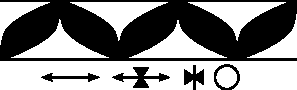
\includegraphics{fpzgrGP.pdf}
\end{array}
\]
This pattern only has symmetry through horizontal translations, glide
reflections, horizontal reflections, and $180^\circ$ rotations. Let
$\mat{T}$ be the horizontal translation, $\mat{G}$ be the glide
reflection, $\mat{F}$ be the horizontal reflection, and $\mat{R}$ be
the $180^\circ$ rotation.

\begin{question} 
Can you express $\mat{T}$ and $\mat{F}$ entirely in terms of $\mat{G}$
and $\mat{R}$?
\end{question}

\begin{question} Is $\mat{G}\mat{R} = \mat{R}\mat{G}$?
\end{question}


\begin{question}
An arbitrary element of $\Zt$ looks like $\mat{T}^n$. An arbitrary
element of $\Zg$ looks like $\mat{G}^n$. What does an arbitrary element
of $\Zgr$ look like?
\end{question}










\subsection{The group $\boldsymbol{\Ztfr}$}

The symmetries of the following frieze pattern form the group $\Ztfr$:\index{ZTRF@$\Ztfr$}
\[
\text{\huge $\Ztfr$:}\qquad\begin{array}{c}
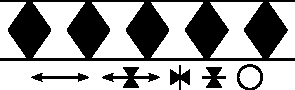
\includegraphics{fptfrGP.pdf}
\end{array}
\]
This pattern has symmetry through horizontal translations, glide
reflections, horizontal reflections, vertical reflections and
$180^\circ$ rotations.  Let $\mat{T}$ be the horizontal translation,
$\mat{G}$ be the glide reflection, $\mat{F_h}$ be the horizontal
reflection, $\mat{F_v}$ be the vertical reflection, and $\mat{R}$ be
the $180^\circ$ rotation.


\begin{question} 
Can you express $\mat{G}$ and $\mat{F_h}$ entirely in terms of $\mat{T}$, $\mat{F_v}$, and $\mat{R}$?
\end{question}

\begin{question} 
Is $\mat{T}\mat{F_v} = \mat{F_v}\mat{T}$? What about $\mat{T}\mat{R} =
\mat{R}\mat{T}$? What about $\mat{F_v}\mat{R} = \mat{R}\mat{F_v}$?
\end{question}

\begin{question}
An arbitrary element of $\Zt$ looks like $\mat{T}^n$. An arbitrary
element of $\Zg$ looks like $\mat{G}^n$. What does an arbitrary element
of $\Ztfr$ look like?
\end{question}


\paragraph{Some observations and thoughts}
As a gesture of friendship, here is a collection of the frieze groups
along with frieze patterns:
\[
{
\renewcommand{\arraystretch}{4}
\begin{array}{c}
\text{\huge $\Zt$:}\qquad\begin{array}{c}
\includegraphics{fptransGP.pdf}
\end{array}\\
\text{\huge $\Zg$:}\qquad\begin{array}{c}
\includegraphics{fpglideGP.pdf}
\end{array}\\
\text{\huge $\Zgf$:}\qquad\begin{array}{c}
\includegraphics{fpverticalGP.pdf}
\end{array}\\
\text{\huge $\Ztf$:}\qquad\begin{array}{c}
\includegraphics{fphorizGP.pdf}
\end{array}\\
\text{\huge $\Ztr$:}\qquad\begin{array}{c}
\includegraphics{fprotGP.pdf}
\end{array}\\
\text{\huge $\Zgr$:}\qquad\begin{array}{c}
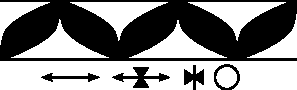
\includegraphics{fpzgrGP.pdf}
\end{array}\\
\text{\huge $\Ztfr$:}\qquad\begin{array}{c}
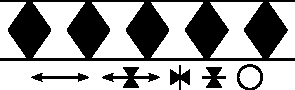
\includegraphics{fptfrGP.pdf}
\end{array}
\end{array}
}
\]










\end{document}
